%%%%%%%%%%%%%%%%%%%%%%%%%%%%%%%%%%%%%%%%%%%%%%%%%%%%%%%%%%%%%%%%%%%%%%%%%%%%%%%%
%2345678901234567890123456789012345678901234567890123456789012345678901234567890
%        1         2         3         4         5         6         7         8

\documentclass[letterpaper, 10 pt, conference]{ieeeconf}  % Comment this line out
                                                          % if you need a4paper
%\documentclass[a4paper, 10pt, conference]{ieeeconf}      % Use this line for a4
                                                          % paper

\IEEEoverridecommandlockouts                              % This command is only
                                                          % needed if you want to
                                                          % use the \thanks command
\overrideIEEEmargins
% See the \addtolength command later in the file to balance the column lengths
% on the last page of the document


\usepackage{graphicx}
\usepackage{minted}

% The following packages can be found on http:\\www.ctan.org
%\usepackage{graphics} % for pdf, bitmapped graphics files
%\usepackage{epsfig} % for postscript graphics files
%\usepackage{mathptmx} % assumes new font selection scheme installed
%\usepackage{times} % assumes new font selection scheme installed
%\usepackage{amsmath} % assumes amsmath package installed
%\usepackage{amssymb}  % assumes amsmath package installed

\title{\LARGE \bf
Embedding Data in 802.11 Beacons for Covert Communication
}

%\author{ \parbox{3 in}{\centering Huibert Kwakernaak*
%         \thanks{*Use the $\backslash$thanks command to put information here}\\
%         Faculty of Electrical Engineering, Mathematics and Computer Science\\
%         University of Twente\\
%         7500 AE Enschede, The Netherlands\\
%         {\tt\small h.kwakernaak@autsubmit.com}}
%         \hspace*{ 0.5 in}
%         \parbox{3 in}{ \centering Pradeep Misra**
%         \thanks{**The footnote marks may be inserted manually}\\
%        Department of Electrical Engineering \\
%         Wright State University\\
%         Dayton, OH 45435, USA\\
%         {\tt\small pmisra@cs.wright.edu}}
%}

\author{Eric Roch$^{1}$% <-this % stops a space
\thanks{$^{1}$Secure and Assured Systems Engineering Intern at Draper 
		and undergraduate at the University of Illinois at Urbana-Champaign. Email:
        {\tt\small eric at roch.us}}%
}


\begin{document}



\maketitle
\thispagestyle{empty}
\pagestyle{empty}


%%%%%%%%%%%%%%%%%%%%%%%%%%%%%%%%%%%%%%%%%%%%%%%%%%%%%%%%%%%%%%%%%%%%%%%%%%%%%%%%
\begin{abstract}

Wireless communications are necessarily observable by anyone within range of the transmitter, making covert wireless communication difficult to conceal.  This paper explores a technique known as Beacon Stuffing, especially as it relates to covert communication in a wireless network, as well as other applications where low-overhead small-data transmissions are required.

\end{abstract}


%%%%%%%%%%%%%%%%%%%%%%%%%%%%%%%%%%%%%%%%%%%%%%%%%%%%%%%%%%%%%%%%%%%%%%%%%%%%%%%%
\section{INTRODUCTION}

At times, information secrecy can be just as important as information security.  Encryption can provide information security - unauthorized individuals will be unable to interpret any information they collect - though it does not provide secrecy, anyone may still monitor the communication.  In times when the simple act of communicating can be just as revealing as the information being shared, it is important that there is no easy way to locate communicating devices.  In a wireless network, all communication is visible to any observer.  However, secrecy does not imply invisibility - communication may still take place on a public channel if an observer is unable to detect it.  The IEEE 802.11 protocol defines several types of network management frames, one of which is a \textit{beacon}, which broadcasts information about the network capabilities of an Access Point (AP).  Beacons are a common sight in wireless network traffic analysis, and as such make for a prime candidate for masking transmissions.  If done correctly, an observer will not know the difference between standard network management traffic and covert communication.

Wireless clients listen for beacon frames to determine which networks are available to join.  To facilitate that decision, beacons contain information about the supported data rates, power levels, and encryption standards. Sometimes it is necessary for AP vendors to include non-standard data specific to the AP.  The 802.11 standard provides a mechanism for this by allowing vendor-specific payloads to be attached to management frames. 

In this paper, we will explore beacon stuffing -- the use of these vendor-specific payloads as a means for transmitting arbitrary data -- with a specific focus on applications where secrecy is desired.


%%%%%%%%%%%%%%%%%%%%%%%%%%%%%%%%%%%%%%%%%%%%%%%%%%%%%%%%%%%%%%%%%%%%%%%%%%%%%%%%
\section{RELATED WORK}

Several other researchers have looked into using beacons as a means for communication. Among these, R. Chandra et al. proposed overloading the Service Set Identifier (SSID), Basic Service Set Identifier (BSSID) and vendor-specific information element (IE) fields \cite{c1}.  Additionally, Gupta and Rohil proposed utilizing unused bits in the length field of each IE \cite{c2}.  The following sections will introduce these techniques and discuss the advantages and shortcomings of each.

\subsection{SSID}

The SSID is a unique identifier of the wireless network. All devices connected to a network must agree on the SSID.  It can be up to 32 alpha-numeric characters, or 32 bytes. R. Chandra et al. proposed using an encoding scheme of a 1 byte message identifier, followed by 1 byte containing a 7-bit fragment counter and a flag indicating more fragments are available, finally followed by the data.  This leaves a maximum of 30 bytes available for data, though the available space will realistically be lower as the base SSID will likely include some identifiable string (i.e. "netXXXXXXXXXXXX...", where XXXXX is the data appended to the original SSID, "net").  Assuming a beacon interval of about 10ms, this gives a maximum data rate of 24 Kbps.

\subsection{BSSID}

The BSSID is a 6 byte field which traditionally represents the media access control (MAC) address of the AP.  However, since the AP MAC address is included in the MAC header of the frame as the transmitter address, this field can be set to any value. By establishing a known SSID, devices may check the BSSID field of matching beacon frames to extract the data. Using the same serialization as before, we can fit 4 data bytes into the BSSID field, giving a transmission rate of 3.2 Kbps.

\subsection{Vendor Information Element}

The 802.11 standard includes a general specification for AP vendors to include up to 253 bytes of data in a special IE.  The format of these information elements is a 3 byte vendor Organizationally Unique Identifier (OUI), a 1 byte vendor-specific type, and up to 252 bytes of data. The IE can either contain the actual OUI with a type to indicate data, providing 252 bytes per frame, or the OUI can be a constant fake value and the type can be used for either data or providing segmentation information.  Again assuming an interval of 10ms, this gives a transmission rate of about 200 Kbps.

\subsection{Information Element Length Field}

Gupta and Rohil proposed a new method, utilizing unused bits in the length field of each IE. Each IE type has a predefined maximum length, some of which require fewer than 8 bits to represent, meaning there are unused bits that are always assumed to be zero.  Firmware modification on the client device would mask out these extra bits to obtain the real length value and reassemble the data using the leftover bits. Based on the table compiled by Gupta and Rohil, this method provides up to 191 bits per frame if every IE is present \cite{c2}. This provides a transmission rate of 19.1 Kbps at a 10ms interval.  Realistically, this will be lower as not every IE will be present.


%%%%%%%%%%%%%%%%%%%%%%%%%%%%%%%%%%%%%%%%%%%%%%%%%%%%%%%%%%%%%%%%%%%%%%%%%%%%%%%%
\section{Comparison of Data Embedding Techniques}

The SSID approach is by far the easiest to implement -- it requires no modification to the drivers on the client or AP. However, most client devices (such as phones, tablets, laptops, etc.) display the SSID to the user for the purpose of selecting a network, which means the data would be visible to the user.  This is not desirable, especially in the context of covert communication, so this approach will not be considered further.

The BSSID offers a promising alternative to the SSID, as it is not client-facing.  Two major limitations are that the BSSID field is not always available (e.g. if the source address is a group address, in which case the BSSID is validated), and it is limited to just 6 bytes per frame \cite{c2}.  Using the BSSID also requires firmware modifications on both the client and AP.

Using the IE length field is an interesting approach and has a considerable advantage in that it utilizes bits that would otherwise go to waste. This means that you can transmit almost 200 bits per frame with no bandwidth cost.  The major limitation is that this method is computationally difficult, requiring separate data structures for storing the locations of these extra bits and preprocessing the whole frame before zeroing out the extra data and passing it on to higher layers. Another drawback is that this method requires modification to the firmware to accommodate future changes to the 802.11 standard which introduce new IE.

The vendor IE approach has the advantage of allowing the most data in a single frame of the methods discussed here, as well as having very little computational cost.  One drawback is that embedding longer data increases frame size, which could congest the network.  However, for the purposes of this paper, we will assume that the data is either short enough to fit in one or two frames, or is not time sensitive and can be buffered until the network is idle. While this method does require firmware modification, the technique is robust and should not be affected by changes to the 802.11 specification.


%%%%%%%%%%%%%%%%%%%%%%%%%%%%%%%%%%%%%%%%%%%%%%%%%%%%%%%%%%%%%%%%%%%%%%%%%%%%%%%%
\section{POTENTIAL APPLICATIONS}

There are numerous potential applications for embedding data in beacon frames.  We will list a variety of them here, but the main focus of this paper is on applications in which the act of communicating must be concealed.

\subsection{Location based advertisements}

Targeted advertising is mutually beneficial to both consumers and marketers.  By narrowing the audience to just those who are likely to act on the advertisement, resources can be used more efficiently.  Location based advertisements are a good way to target a group of people who will likely be interested in a topic, coupon, etc.  However, privacy is a growing concern among users, and using standard location services such as GPS requires either substantial access to the system or an always running application to send location data, neither of which are ideal. Due to the limited range of wireless signals, advertisements served from an AP will only reach devices in the immediate vicinity, thus providing localization without needing to gather user data.

Beacon stuffing can be used to embed advertisement data such that all devices within range of the AP receive the advertisement or coupon.  This would, however, require driver modification in order to present the embedded data to a user.

\subsection{Network monitoring/data extraction}

Since beacon stuffing requires modification of the firmware on the AP, we will assume that we have complete access to the AP, but not necessarily to the networks broadcast by the AP (e.g. a compromised AP).  In such a scenario, we can use beacon stuffing to extract information about a network or specific traffic without showing suspicious traffic.  Special software running on the AP could collect and log data about connected clients and traffic patterns, then dump the log (or a summary) via beacon stuffing on request.  An adversary could use this to gather metadata about a network without ever connecting to it.  Although the actual data transmitted would be secure (assuming some level of transport security), the knowledge of who connects to whom and when could be just as useful.

\subsection{Low-overhead burst communication}

Consider a situation where a group of devices in the same vicinity, but not necessarily on the same network, need to receive information from a central authority at the same time.  One solution would be to send a broadcast or multicast TCP message on each network containing target devices.  This would require the formation of a distinct data frame for each network, which will increase the overhead as more networks are added.  This requires that every device is associated with a network.  Alternatively, we can use beacon stuffing to communicate to all of these devices across multiple networks simultaneously, with fixed overhead.  In such a scenario, we might set up a WLAN called "announcements" which each target device would be able to receive beacons from, even if they are associated with another network.  By stuffing the beacons for this announcements WLAN, all devices in the area can receive the same message with a fixed overhead of a single beacon frame.

\subsection{Covert communication}

In a situation where an agent must receive information from or report back to a supervisor, but the agent cannot risk the discovery of the communication, beacon stuffing can simplify the setup required. If the supervisor can gain control of a public AP, the agent can communicate simply by being in range of the AP without ever connecting or sending any data frames.  In this way, someone trying to identify an undercover agent would need special knowledge of the communication system in order to detect that this communication is taking place.  Without advance knowledge, this would look just like a typical beacon or probe request.  Due to the sheer number of these in a short time frame, manually filtering a network capture is infeasible. A scripted search could be performed, but at that point the attacker knows about the communication channel and we would have to fall back on encryption.


%%%%%%%%%%%%%%%%%%%%%%%%%%%%%%%%%%%%%%%%%%%%%%%%%%%%%%%%%%%%%%%%%%%%%%%%%%%%%%%%
\section{BEACON FRAME FORMAT}

The 802.11 protocol describes a standard format for beacon frames, which are a type of management frame.  Each beacon frame consists of a MAC header, body, and frame check sequence (FCS).  The MAC header contains information such as source and destination addresses, sequence and fragment IDs, and control flags.  The FCS is simply an error detection mechanism that signals the recipient to discard damaged frames.

\begin{figure}[h!]
% 	\centering
    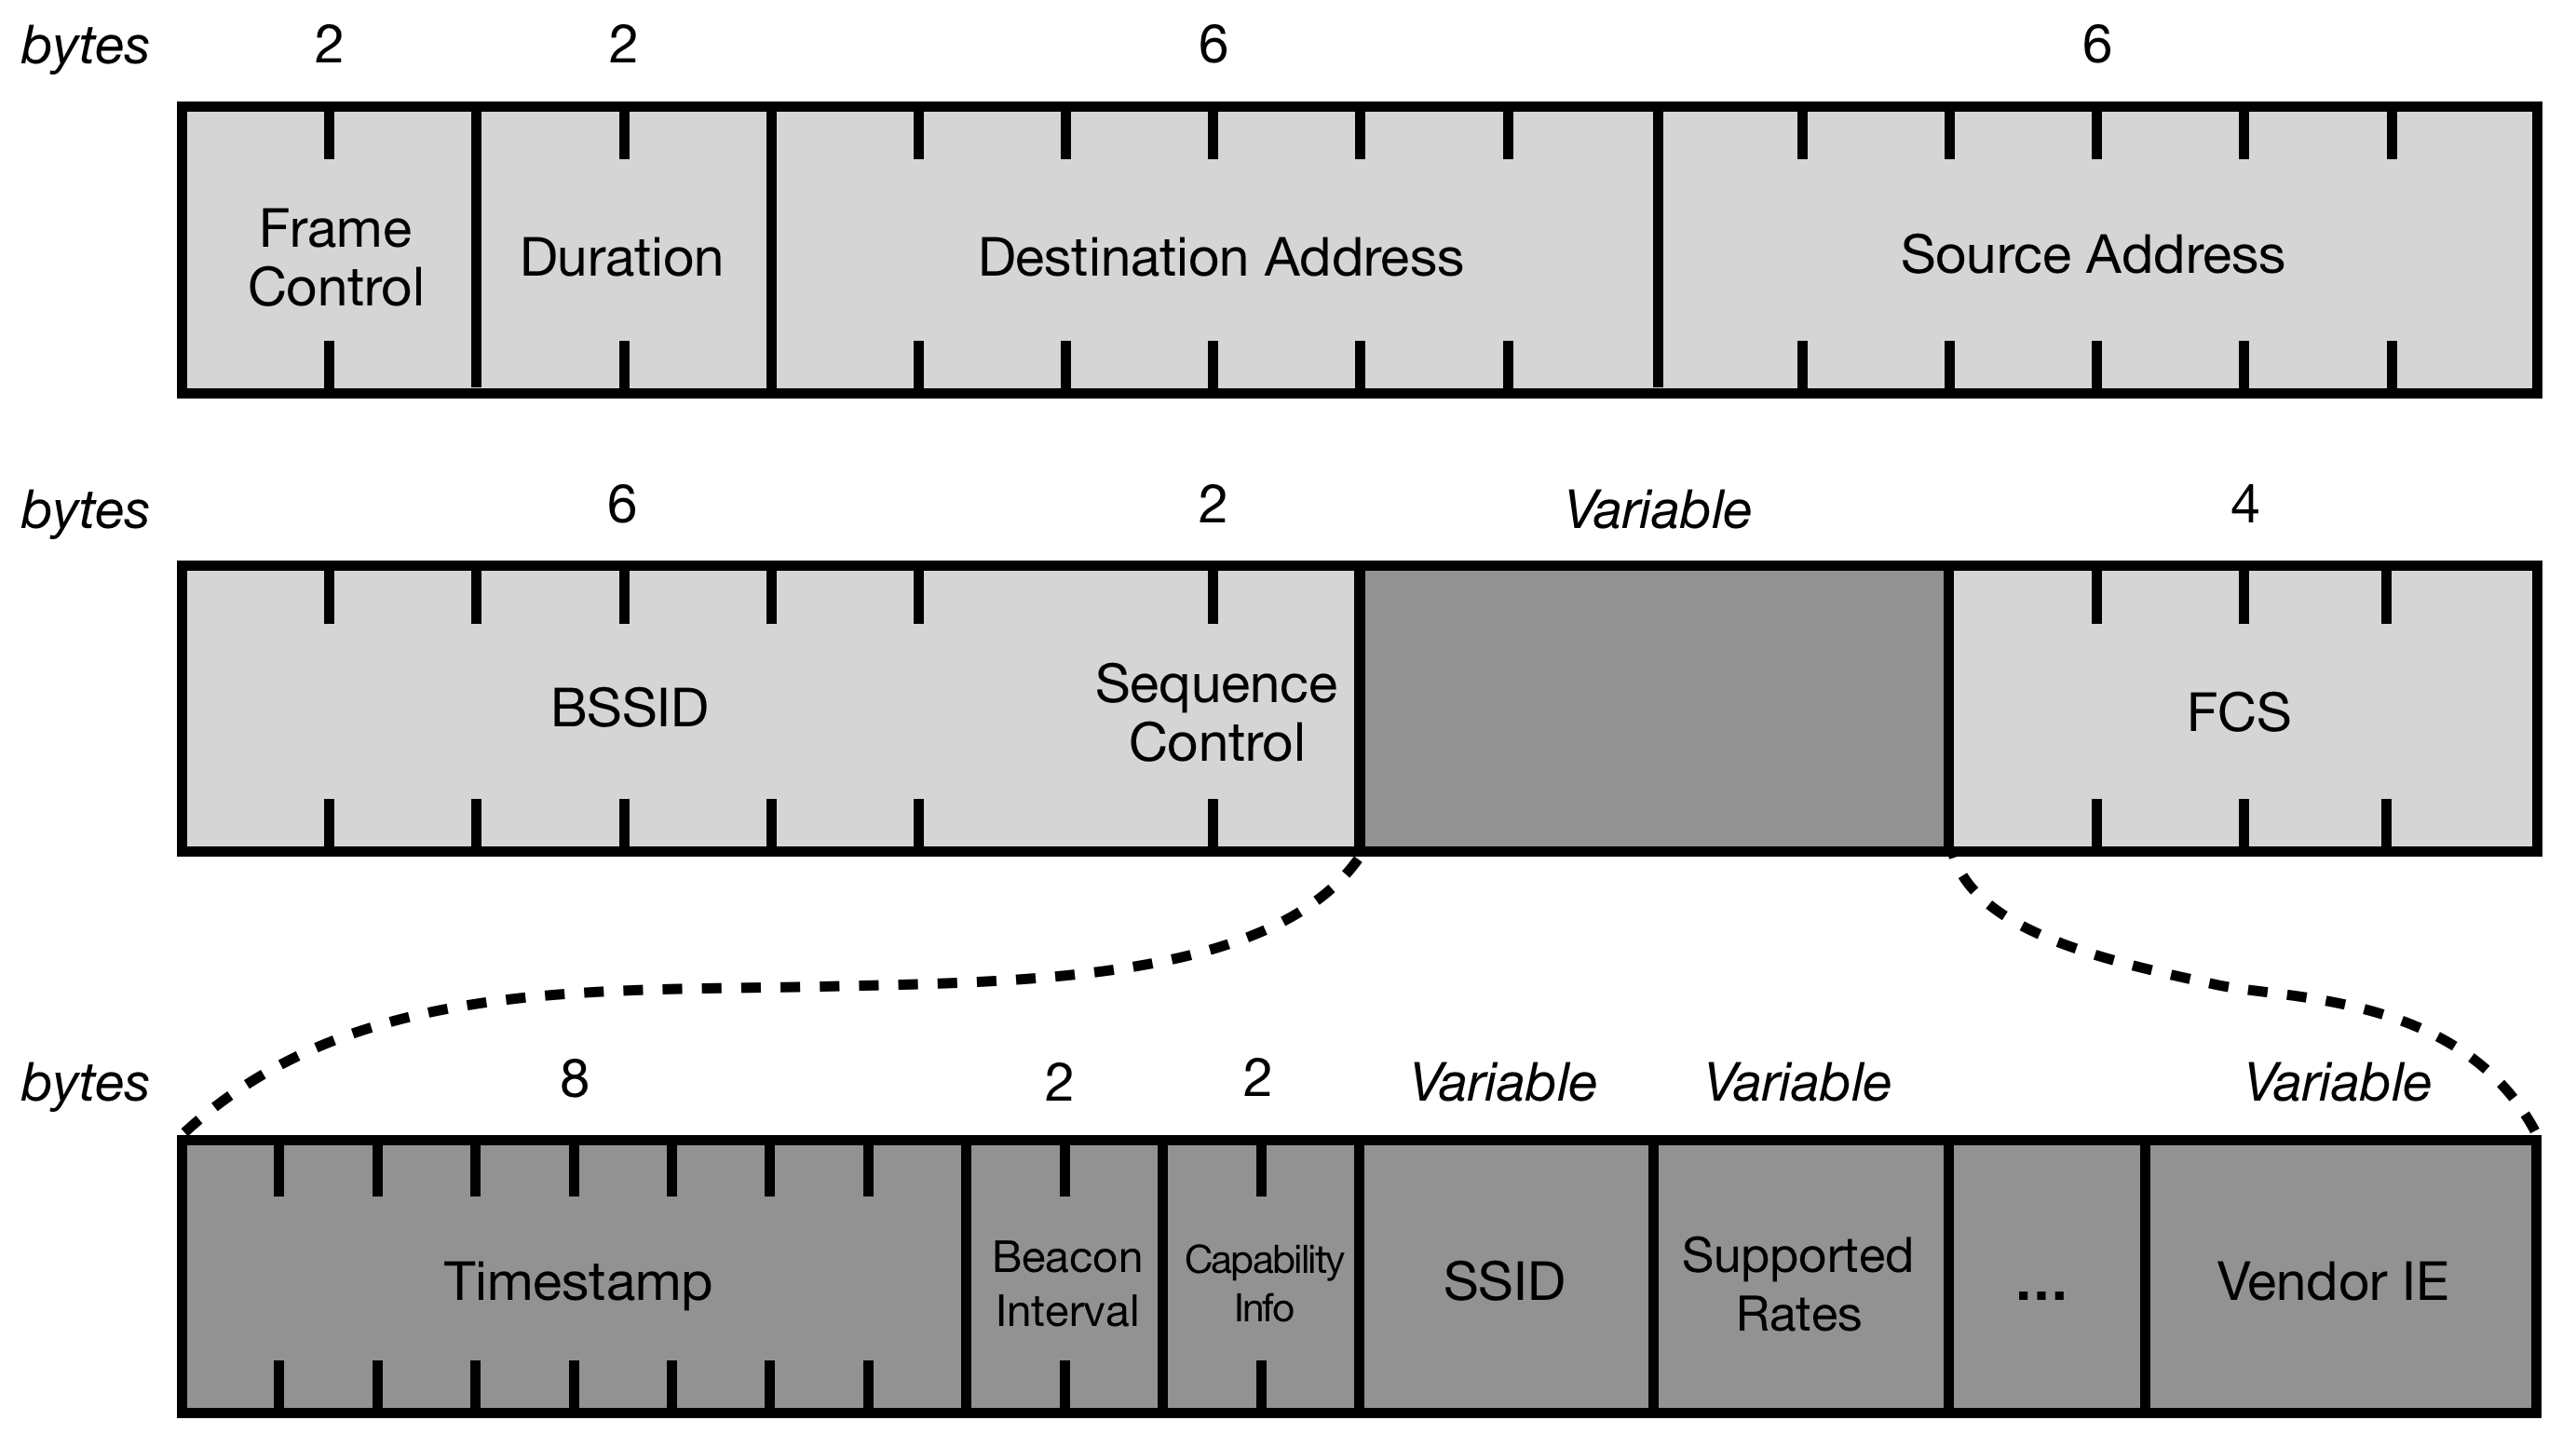
\includegraphics[width=3.25in]{beaconFrame.png}
    \caption{General structure of 802.11 beacon frame.  The MAC header is shown in light gray, the beacon payload is shown in dark gray.}
    \label{fig:beacon}
\end{figure}

The body of a beacon frame is made up of several required fields and IE, and may contain additional IE.  The required fields are timestamp, interval, and capabilities, followed by two IE containing the SSID and supported rates. The body may then contain more IE, up to a total frame size of 2304 bytes. Each IE can be up to 257 bytes, containing a 1 byte ID, 1 byte length field, and $N$ data bytes, where $N$ is the value in the length field.  For the vendor IE, the first 4 data bytes are the vendor's OUI and a type specifier, as shown in Figure \ref{fig:vendorIE}.

\begin{figure}[h!]
% 	\centering
	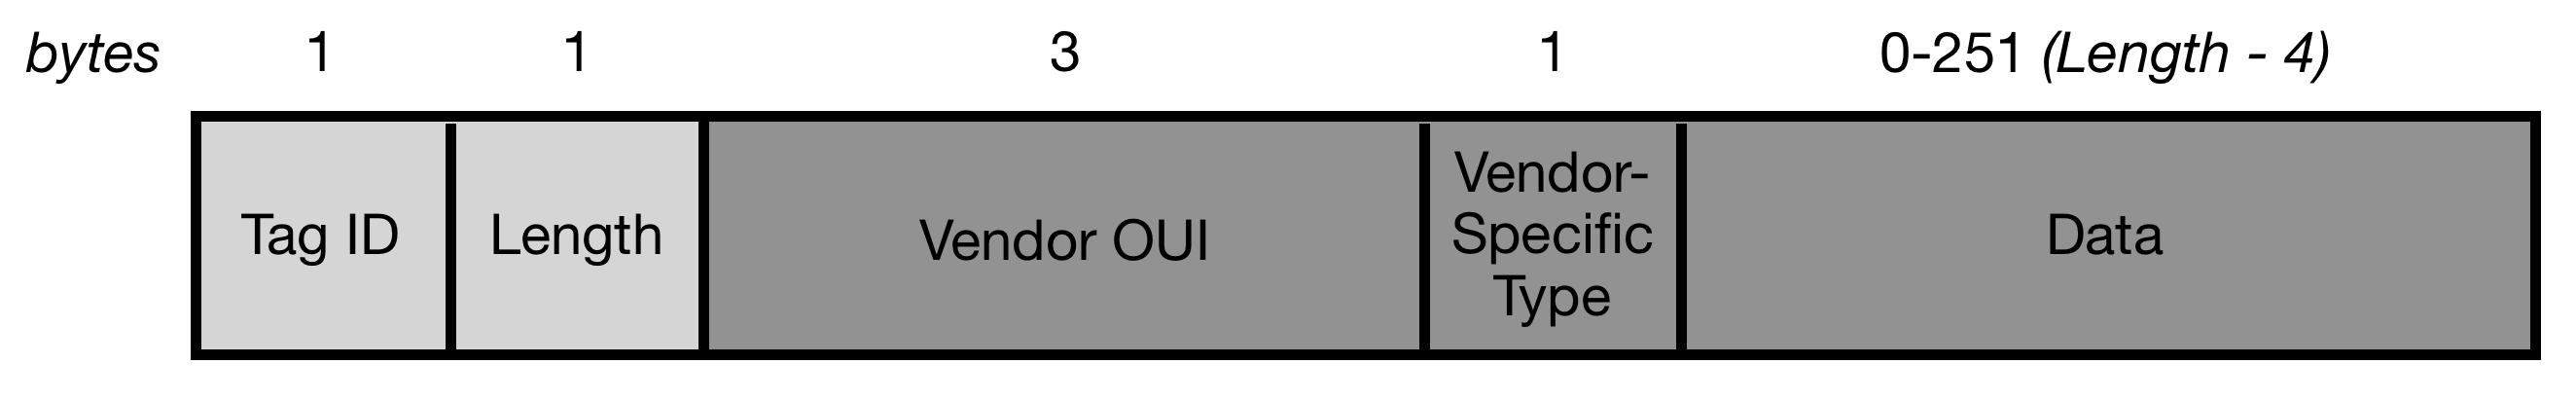
\includegraphics[width=3.25in]{vendorIE.png}
    \caption{Structure of Vendor-Specific IE}
    \label{fig:vendorIE}
\end{figure}


%%%%%%%%%%%%%%%%%%%%%%%%%%%%%%%%%%%%%%%%%%%%%%%%%%%%%%%%%%%%%%%%%%%%%%%%%%%%%%%
\section{IMPLEMENTATION}

As a proof-of-concept to show that beacon stuffing is feasible, we will explore a simple implementation that utilizes the vendor IE.  For sake of brevity and simplicity, we will only consider one AP chipset, the Ralink RT3070L, connected via USB to an Ubuntu host.  The only requirement for this demonstration is that the transmitter chipset supports packet injection.  This should otherwise be completely general.

\subsection{Data Protection}

Some applications of beacon stuffing may require the data to be secure and most will want some form of integrity check to prevent malicious inspection or modification of the data.  For this example, we will use a symmetric encryption scheme from the Python Cryptography package known as Fernet encryption, which utilizes AES-128-CBC for encryption and SHA256 based HMAC for integrity \cite{c5}.  To use this, we encrypt the message before constructing the beacon. This will be discussed more in the Results and Considerations section.

\subsection{Frame Creation}

While it does not matter how the frame is actually created (it could be written directly in binary), we will use a Python library called Scapy \cite{c4} to assist with frame creation.

To generate a stuffed beacon frame, we first create a basic frame containing the MAC header.  We then split the message into chunks of 251 bytes, if neccessary, and embed them into vendor IE which are then attached to the base frame as a payload.  If there were multiple chunks, we have a fragmented frame, so we will use the MAC header's \textit{fragment ID} field and \textit{More Fragments} flag to indicate to the receiver that the message is fragmented.

\subsection{Message Recovery}

To recover the original message, we must first record the transmitted beacons.  This is easy to do using Wireshark \cite{c6} another computer.  By saving a packet capture file which contains our custom beacon, we can use Scapy and Python again to filter the file and recover the message.  We start by loading the saved capture file, then apply a filter based on some criteria which are unique to our beacons.  This could be an SSID (such as "announcements"), a BSSID, or a special IE.  After obtaining a filtered list of just the stuffed packets, we can dissect them to extract the IE containing our message.  We will store the extracted message pieces in a dictionary keyed with the fragment ID of the packet, which allows us to reconstruct the original message if the beacons are out of order and to determine if any pieces are missing.  Once reassembled, the message can be decrypted and processed.


%%%%%%%%%%%%%%%%%%%%%%%%%%%%%%%%%%%%%%%%%%%%%%%%%%%%%%%%%%%%%%%%%%%%%%%%%%%%%%%
\section{RESULTS AND CONSIDERATIONS}



%%%%%%%%%%%%%%%%%%%%%%%%%%%%%%%%%%%%%%%%%%%%%%%%%%%%%%%%%%%%%%%%%%%%%%%%%%%%%%%
\section{FUTURE WORK}




\newpage
%%%%%%%%%%%%%%%%%%%%%%%%%%%%%%%%%%%%%%%%%%%%%%%%%%%%%%%%%%%%%%%%%%%%%%%%%%%%%%%%
% \section{SECTION TITLE}

% \subsection{Selecting a Template (Heading 2)}

% First, confirm that you have the correct template for your paper size. This template has been tailored for output on the US-letter paper size. Please do not use it for A4 paper since the margin requirements for A4 papers may be different from Letter paper size.

% \subsection{Maintaining the Integrity of the Specifications}

% The template is used to format your paper and style the text. All margins, column widths, line spaces, and text fonts are prescribed; please do not alter them. You may note peculiarities. For example, the head margin in this template measures proportionately more than is customary. This measurement and others are deliberate, using specifications that anticipate your paper as one part of the entire proceedings, and not as an independent document. Please do not revise any of the current designations

% \section{MATH}

% Before you begin to format your paper, first write and save the content as a separate text file. Keep your text and graphic files separate until after the text has been formatted and styled. Do not use hard tabs, and limit use of hard returns to only one return at the end of a paragraph. Do not add any kind of pagination anywhere in the paper. Do not number text heads-the template will do that for you.

% Finally, complete content and organizational editing before formatting. Please take note of the following items when proofreading spelling and grammar:

% \subsection{Abbreviations and Acronyms} Define abbreviations and acronyms the first time they are used in the text, even after they have been defined in the abstract. Abbreviations such as IEEE, SI, MKS, CGS, sc, dc, and rms do not have to be defined. Do not use abbreviations in the title or heads unless they are unavoidable.

% \subsection{Units}

% \begin{itemize}

% \item Use either SI (MKS) or CGS as primary units. (SI units are encouraged.) English units may be used as secondary units (in parentheses). An exception would be the use of English units as identifiers in trade, such as Ò3.5-inch disk driveÓ.
% \item Avoid combining SI and CGS units, such as current in amperes and magnetic field in oersteds. This often leads to confusion because equations do not balance dimensionally. If you must use mixed units, clearly state the units for each quantity that you use in an equation.
% \item Do not mix complete spellings and abbreviations of units: ÒWb/m2Ó or Òwebers per square meterÓ, not Òwebers/m2Ó.  Spell out units when they appear in text: Ò. . . a few henriesÓ, not Ò. . . a few HÓ.
% \item Use a zero before decimal points: Ò0.25Ó, not Ò.25Ó. Use Òcm3Ó, not ÒccÓ. (bullet list)

% \end{itemize}


% \subsection{Equations}

% The equations are an exception to the prescribed specifications of this template. You will need to determine whether or not your equation should be typed using either the Times New Roman or the Symbol font (please no other font). To create multileveled equations, it may be necessary to treat the equation as a graphic and insert it into the text after your paper is styled. Number equations consecutively. Equation numbers, within parentheses, are to position flush right, as in (1), using a right tab stop. To make your equations more compact, you may use the solidus ( / ), the exp function, or appropriate exponents. Italicize Roman symbols for quantities and variables, but not Greek symbols. Use a long dash rather than a hyphen for a minus sign. Punctuate equations with commas or periods when they are part of a sentence, as in

% $$
% \alpha + \beta = \chi \eqno{(1)}
% $$

% Note that the equation is centered using a center tab stop. Be sure that the symbols in your equation have been defined before or immediately following the equation. Use Ò(1)Ó, not ÒEq. (1)Ó or Òequation (1)Ó, except at the beginning of a sentence: ÒEquation (1) is . . .Ó

% \subsection{Some Common Mistakes}
% \begin{itemize}


% \item The word ÒdataÓ is plural, not singular.
% \item The subscript for the permeability of vacuum ?0, and other common scientific constants, is zero with subscript formatting, not a lowercase letter ÒoÓ.
% \item In American English, commas, semi-/colons, periods, question and exclamation marks are located within quotation marks only when a complete thought or name is cited, such as a title or full quotation. When quotation marks are used, instead of a bold or italic typeface, to highlight a word or phrase, punctuation should appear outside of the quotation marks. A parenthetical phrase or statement at the end of a sentence is punctuated outside of the closing parenthesis (like this). (A parenthetical sentence is punctuated within the parentheses.)
% \item A graph within a graph is an ÒinsetÓ, not an ÒinsertÓ. The word alternatively is preferred to the word ÒalternatelyÓ (unless you really mean something that alternates).
% \item Do not use the word ÒessentiallyÓ to mean ÒapproximatelyÓ or ÒeffectivelyÓ.
% \item In your paper title, if the words Òthat usesÓ can accurately replace the word ÒusingÓ, capitalize the ÒuÓ; if not, keep using lower-cased.
% \item Be aware of the different meanings of the homophones ÒaffectÓ and ÒeffectÓ, ÒcomplementÓ and ÒcomplimentÓ, ÒdiscreetÓ and ÒdiscreteÓ, ÒprincipalÓ and ÒprincipleÓ.
% \item Do not confuse ÒimplyÓ and ÒinferÓ.
% \item The prefix ÒnonÓ is not a word; it should be joined to the word it modifies, usually without a hyphen.
% \item There is no period after the ÒetÓ in the Latin abbreviation Òet al.Ó.
% \item The abbreviation Òi.e.Ó means Òthat isÓ, and the abbreviation Òe.g.Ó means Òfor exampleÓ.

% \end{itemize}


% \section{USING THE TEMPLATE}

% Use this sample document as your LaTeX source file to create your document. Save this file as {\bf root.tex}. You have to make sure to use the cls file that came with this distribution. If you use a different style file, you cannot expect to get required margins. Note also that when you are creating your out PDF file, the source file is only part of the equation. {\it Your \TeX\ $\rightarrow$ PDF filter determines the output file size. Even if you make all the specifications to output a letter file in the source - if you filter is set to produce A4, you will only get A4 output. }

% It is impossible to account for all possible situation, one would encounter using \TeX. If you are using multiple \TeX\ files you must make sure that the ``MAIN`` source file is called root.tex - this is particularly important if your conference is using PaperPlaza's built in \TeX\ to PDF conversion tool.

% \subsection{Headings, etc}

% Text heads organize the topics on a relational, hierarchical basis. For example, the paper title is the primary text head because all subsequent material relates and elaborates on this one topic. If there are two or more sub-topics, the next level head (uppercase Roman numerals) should be used and, conversely, if there are not at least two sub-topics, then no subheads should be introduced. Styles named ÒHeading 1Ó, ÒHeading 2Ó, ÒHeading 3Ó, and ÒHeading 4Ó are prescribed.

% \subsection{Figures and Tables}

% Positioning Figures and Tables: Place figures and tables at the top and bottom of columns. Avoid placing them in the middle of columns. Large figures and tables may span across both columns. Figure captions should be below the figures; table heads should appear above the tables. Insert figures and tables after they are cited in the text. Use the abbreviation ÒFig. 1Ó, even at the beginning of a sentence.

% \begin{table}[h]
% \caption{An Example of a Table}
% \label{table_example}
% \begin{center}
% \begin{tabular}{|c||c|}
% \hline
% One & Two\\
% \hline
% Three & Four\\
% \hline
% \end{tabular}
% \end{center}
% \end{table}


%    \begin{figure}[thpb]
%       \centering
%       \framebox{\parbox{3in}{We suggest that you use a text box to insert a graphic (which is ideally a 300 dpi TIFF or EPS file, with all fonts embedded) because, in an document, this method is somewhat more stable than directly inserting a picture.
% }}
%       %\includegraphics[scale=1.0]{figurefile}
%       \caption{Inductance of oscillation winding on amorphous
%        magnetic core versus DC bias magnetic field}
%       \label{figurelabel}
%    \end{figure}
   

% Figure Labels: Use 8 point Times New Roman for Figure labels. Use words rather than symbols or abbreviations when writing Figure axis labels to avoid confusing the reader. As an example, write the quantity ÒMagnetizationÓ, or ÒMagnetization, MÓ, not just ÒMÓ. If including units in the label, present them within parentheses. Do not label axes only with units. In the example, write ÒMagnetization (A/m)Ó or ÒMagnetization {A[m(1)]}Ó, not just ÒA/mÓ. Do not label axes with a ratio of quantities and units. For example, write ÒTemperature (K)Ó, not ÒTemperature/K.Ó

% \section{CONCLUSIONS}

% A conclusion section is not required. Although a conclusion may review the main points of the paper, do not replicate the abstract as the conclusion. A conclusion might elaborate on the importance of the work or suggest applications and extensions. 

% \addtolength{\textheight}{-12cm}   % This command serves to balance the column lengths
                                  % on the last page of the document manually. It shortens
                                  % the textheight of the last page by a suitable amount.
                                  % This command does not take effect until the next page
                                  % so it should come on the page before the last. Make
                                  % sure that you do not shorten the textheight too much.

%%%%%%%%%%%%%%%%%%%%%%%%%%%%%%%%%%%%%%%%%%%%%%%%%%%%%%%%%%%%%%%%%%%%%%%%%%%%%%%%



%%%%%%%%%%%%%%%%%%%%%%%%%%%%%%%%%%%%%%%%%%%%%%%%%%%%%%%%%%%%%%%%%%%%%%%%%%%%%%%%



%%%%%%%%%%%%%%%%%%%%%%%%%%%%%%%%%%%%%%%%%%%%%%%%%%%%%%%%%%%%%%%%%%%%%%%%%%%%%%%%
% \section*{APPENDIX}

% Appendixes should appear before the acknowledgment.

% \section*{ACKNOWLEDGMENT}

% The preferred spelling of the word ÒacknowledgmentÓ in America is without an ÒeÓ after the ÒgÓ. Avoid the stilted expression, ÒOne of us (R. B. G.) thanks . . .Ó  Instead, try ÒR. B. G. thanksÓ. Put sponsor acknowledgments in the unnumbered footnote on the first page.



% %%%%%%%%%%%%%%%%%%%%%%%%%%%%%%%%%%%%%%%%%%%%%%%%%%%%%%%%%%%%%%%%%%%%%%%%%%%%%%%%

% References are important to the reader; therefore, each citation must be complete and correct. If at all possible, references should be commonly available publications.



\begin{thebibliography}{99}

\bibitem{c1} R. Chandra, J. Padhye, L. Ravindranath, and A. Wolman, “Beacon-Stuffing: Wi-Fi without Associations,” \textit{Eighth IEEE Workshop on Mobile Computing Systems and Applications}, 2007.
\bibitem{c2} V. Gupta and M. K. Rohil, “Bit-Stuffing in 802. 11 Beacon Frame: Embedding Non-Standard Custom Information,” \textit{International Journal of Computer Applications}, vol. 63, no. 2, pp. 6–12, Feb. 2013.
\bibitem{c3} M. S. Gast, \textit{802.11 Wireless Networks: The Definitive Guide}, 2nd ed. Beijing: O'Reilly, 2013.
\bibitem{c4} P. Biondi, “Scapy,” \textit{Scapy}. [Online]. Available: https://scapy.net/. [Accessed: 02-Aug-2018].
\bibitem{c5} “Fernet (symmetric encryption),” \textit{Welcome to pyca/cryptography}. [Online]. Available: https://cryptography.io/en/latest/fernet/. [Accessed: 02-Aug-2018].
\bibitem{c6} “Wireshark,” \textit{Wireshark Documentation}. [Online]. Available: https://www.wireshark.org/. [Accessed: 02-Aug-2018].
% \bibitem{c7} C. J. Kaufman, Rocky Mountain Research Lab., Boulder, CO, private communication, May 1995.
% \bibitem{c8} Y. Yorozu, M. Hirano, K. Oka, and Y. Tagawa, ÒElectron spectroscopy studies on magneto-optical media and plastic substrate interfaces(Translation Journals style),Ó IEEE Transl. J. Magn.Jpn., vol. 2, Aug. 1987, pp. 740Ð741 [Dig. 9th Annu. Conf. Magnetics Japan, 1982, p. 301].
% \bibitem{c9} M. Young, The Techincal Writers Handbook.  Mill Valley, CA: University Science, 1989.
% \bibitem{c10} J. U. Duncombe, ÒInfrared navigationÑPart I: An assessment of feasibility (Periodical style),Ó IEEE Trans. Electron Devices, vol. ED-11, pp. 34Ð39, Jan. 1959.
% \bibitem{c11} S. Chen, B. Mulgrew, and P. M. Grant, ÒA clustering technique for digital communications channel equalization using radial basis function networks,Ó IEEE Trans. Neural Networks, vol. 4, pp. 570Ð578, July 1993.
% \bibitem{c12} R. W. Lucky, ÒAutomatic equalization for digital communication,Ó Bell Syst. Tech. J., vol. 44, no. 4, pp. 547Ð588, Apr. 1965.
% \bibitem{c13} S. P. Bingulac, ÒOn the compatibility of adaptive controllers (Published Conference Proceedings style),Ó in Proc. 4th Annu. Allerton Conf. Circuits and Systems Theory, New York, 1994, pp. 8Ð16.
% \bibitem{c14} G. R. Faulhaber, ÒDesign of service systems with priority reservation,Ó in Conf. Rec. 1995 IEEE Int. Conf. Communications, pp. 3Ð8.
% \bibitem{c15} W. D. Doyle, ÒMagnetization reversal in films with biaxial anisotropy,Ó in 1987 Proc. INTERMAG Conf., pp. 2.2-1Ð2.2-6.
% \bibitem{c16} G. W. Juette and L. E. Zeffanella, ÒRadio noise currents n short sections on bundle conductors (Presented Conference Paper style),Ó presented at the IEEE Summer power Meeting, Dallas, TX, June 22Ð27, 1990, Paper 90 SM 690-0 PWRS.
% \bibitem{c17} J. G. Kreifeldt, ÒAn analysis of surface-detected EMG as an amplitude-modulated noise,Ó presented at the 1989 Int. Conf. Medicine and Biological Engineering, Chicago, IL.
% \bibitem{c18} J. Williams, ÒNarrow-band analyzer (Thesis or Dissertation style),Ó Ph.D. dissertation, Dept. Elect. Eng., Harvard Univ., Cambridge, MA, 1993. 
% \bibitem{c19} N. Kawasaki, ÒParametric study of thermal and chemical nonequilibrium nozzle flow,Ó M.S. thesis, Dept. Electron. Eng., Osaka Univ., Osaka, Japan, 1993.
% \bibitem{c20} J. P. Wilkinson, ÒNonlinear resonant circuit devices (Patent style),Ó U.S. Patent 3 624 12, July 16, 1990. 

\end{thebibliography}




\end{document}
